\documentclass{standalone}
\usepackage{tikz}
\usetikzlibrary{arrows.meta}
\usetikzlibrary{snakes}
\usetikzlibrary{patterns}

%: === TIPOGRAFÍA === (((
\usepackage{fontspec}
\setmainfont[
  BoldFont       = bodonibi,
	ItalicFont     = Century modern italic2.ttf,
	BoldItalicFont = bodonibi,
	SmallCapsFont  = lmromancaps10-regular.otf
]{Century_modern.ttf}
\DeclareSymbolFont{italics}{\encodingdefault}{\rmdefault}{m}{it}
\DeclareSymbolFontAlphabet{\mathit}{italics}
\ExplSyntaxOn
\int_step_inline:nnnn { `A } { 1 } { `Z }
 {  \exp_args:Nf \DeclareMathSymbol{\char_generate:nn{#1}{11}}{\mathalpha}{italics}{#1} }
\int_step_inline:nnnn { `a } { 1 } { `z } {  \exp_args:Nf \DeclareMathSymbol{\char_generate:nn{#1}{11}}{\mathalpha}{italics}{#1}}
\ExplSyntaxOff
% )))

\begin{document}

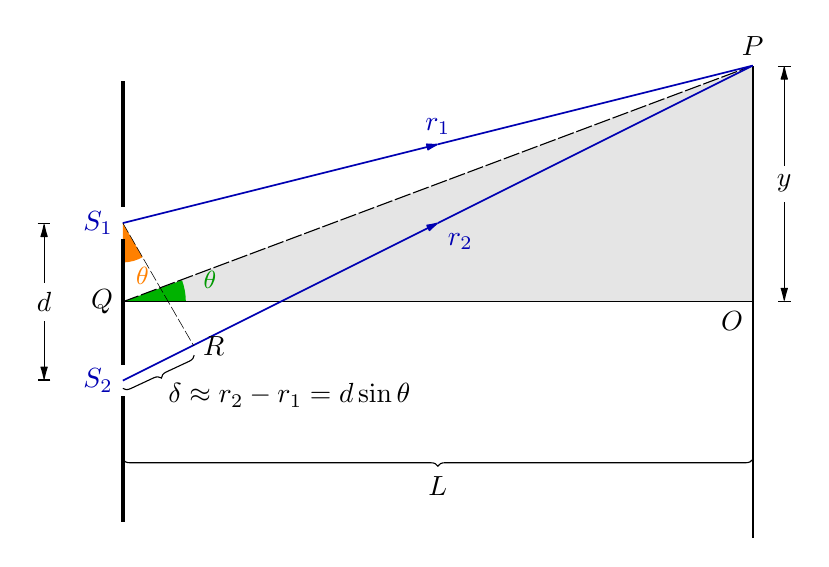
\begin{tikzpicture}[>={Latex[round,width=1mm,length=2mm]}, scale=2]
	\fill [black!10] (0,1.5) -- (4,1.5) -- (4,3) -- cycle;
	\fill [green!70!black] (0,1.5) --++ (4mm,0) arc (0:20: 4mm) node [right=1.5mm, green!60!black] {\small \(\theta\)} -- cycle;
	\fill [orange] (0,2) --++ (0,-2.5mm) arc (-90:-60: 2.5mm) node [below] {\small \(\theta\)} -- cycle;
	\draw [ultra thick] (0,2.9) -- (0,2.1) (0,1.9) -- (0,1.1) (0,0.9) -- (0,0.1); 
	\draw (0,1.5) node [left] { \(Q\)} --++ (4,0) node [below left] {\(O\)};
	\draw [|<->|] (-0.5,2) to node [midway,fill=white] { \(d\)} (-0.5,1);
	\draw [dash pattern = on 6pt off 1pt] (0,1.5) --++ (4,1.5) node [above] {\(P\)};
	\draw [semithick] (4,0) -- (4,3);
	\draw [|<->|] (4.2,1.5) to node[midway,fill=white] { \(y\)} (4.2,3);
	\draw [blue!70!black,semithick] (2,2) -- (4,3);
	\draw [blue!70!black,-{Latex[round,width=1mm, length=2mm]}, semithick] (0,1) node [left] { \(S_2\)} -- (2,2) node [below right] { \(r_{2}\)};
	\draw [blue!70!black,-{Latex[round,width=1mm, length=2mm]}, semithick] (0,2) node [left] { \(S_1\)} -- (2,2.5) node [above] { \(r_{1}\)};
	\draw [blue!70!black,semithick] (2,2.5) -- (4,3);
	\draw [dash pattern = on 4pt off 1pt, very thin] (0,2) --++ (-60:9mm) node [right] {\(R\)};
	\draw [snake = brace, mirror snake] (0,0.5) to node[midway,below = 1mm] {\(L\)} ++ (4,0);
	\draw [snake = brace, mirror snake] (0,0.95) to node[midway, below = 3mm, right=0mm] {\(\delta \approx r_2-r_1 = d \sin \theta\)} ++ (25:0.5cm);
\end{tikzpicture}

\end{document}
